\documentclass[a4paper]{article}
\usepackage[spanish]{babel}
\usepackage[utf8]{inputenc}
\usepackage{charter}   % tipografia
\usepackage{graphicx}
%\usepackage{makeidx}

%\usepackage{float}
%\usepackage{amsmath, amsthm, amssymb}
%\usepackage{amsfonts}
%\usepackage{sectsty}
%\usepackage{charter}
%\usepackage{wrapfig}
%\usepackage{listings}
%\lstset{language=C}


\usepackage{color} % para snipets de codigo coloreados
\usepackage{fancybox}  % para el sbox de los snipets de codigo

\definecolor{litegrey}{gray}{0.94}

% \newenvironment{sidebar}{%
% 	\begin{Sbox}\begin{minipage}{.85\textwidth}}%
% 	{\end{minipage}\end{Sbox}%
% 		\begin{center}\setlength{\fboxsep}{6pt}%
% 		\shadowbox{\TheSbox}\end{center}}
% \newenvironment{warning}{%
% 	\begin{Sbox}\begin{minipage}{.85\textwidth}\sffamily\lite\small\RaggedRight}%
% 	{\end{minipage}\end{Sbox}%
% 		\begin{center}\setlength{\fboxsep}{6pt}%
% 		\colorbox{litegrey}{\TheSbox}\end{center}}

\newenvironment{codesnippet}{%
	\begin{Sbox}\begin{minipage}{\textwidth}\sffamily\small}%
	{\end{minipage}\end{Sbox}%
		\begin{center}%
		\colorbox{litegrey}{\TheSbox}\end{center}}



\usepackage{fancyhdr}
\pagestyle{fancy}

%\renewcommand{\chaptermark}[1]{\markboth{#1}{}}
\renewcommand{\sectionmark}[1]{\markright{\thesection\ - #1}}

\fancyhf{}

\fancyhead[LO]{Sección \rightmark} % \thesection\ 
\fancyfoot[LO]{\small{Nombre Apellido, Nombre Apellido, Nombre Apellido}}
\fancyfoot[RO]{\thepage}
\renewcommand{\headrulewidth}{0.5pt}
\renewcommand{\footrulewidth}{0.5pt}
\setlength{\hoffset}{-0.8in}
\setlength{\textwidth}{16cm}
%\setlength{\hoffset}{-1.1cm}
%\setlength{\textwidth}{16cm}
\setlength{\headsep}{0.5cm}
\setlength{\textheight}{25cm}
\setlength{\voffset}{-0.7in}
\setlength{\headwidth}{\textwidth}
\setlength{\headheight}{13.1pt}

\renewcommand{\baselinestretch}{1.1}  % line spacing


% \setcounter{secnumdepth}{2}
\usepackage{underscore}
\usepackage{caratula}
\usepackage{url}


% ******************************************************** %
%              TEMPLATE DE INFORME ORGA2 v0.1              %
% ******************************************************** %
% ******************************************************** %
%                                                          %
% ALGUNOS PAQUETES REQUERIDOS (EN UBUNTU):                 %
% ========================================
%                                                          %
% texlive-latex-base                                       %
% texlive-latex-recommended                                %
% texlive-fonts-recommended                                %
% texlive-latex-extra?                                     %
% texlive-lang-spanish (en ubuntu 13.10)                   %
% ******************************************************** %



\begin{document}


\thispagestyle{empty}
\materia{Organización del Computador II}
\submateria{Primer Cuatrimestre de 2014}
\titulo{Trabajo Práctico II}
\subtitulo{subtitulo del trabajo}
\integrante{Nombre}{XXX/XX}{mail}
\integrante{Nombre}{XXX/XX}{mail}

\maketitle
\newpage

\thispagestyle{empty}
\vfill
\begin{abstract}
En el presente trabajo se describe la problemática de ...
\end{abstract}

\thispagestyle{empty}
\vspace{3cm}
\tableofcontents
\newpage


%\normalsize
\newpage

\section{Objetivos generales}

El objetivo de este Trabajo Práctico es ...


\section{Contexto}

\begin{figure}
  \begin{center}
	
\includegraphics[scale=0.66]{imagenes/logouba.jpg}
	\caption{Descripcion de la figura}
	\label{nombreparareferenciar}
  \end{center}
\end{figure}


\paragraph{\textbf{Titulo del parrafo} } Bla bla bla bla.
Esto se muestra en la figura~\ref{nombreparareferenciar}.



\begin{codesnippet}
\begin{verbatim}

struct Pepe {

    ...

};

\end{verbatim}
\end{codesnippet}


\section{Enunciado y solucion} 
\subsection*{Filtro \textit{tiles}}

Programar el filtro \textit{tiles} en lenguaje C y luego en ASM haciendo uso de las instrucciones vectoriales (\textbf{SSE}).
    

\vspace*{0.3cm} \noindent
\textbf{Descripción}

En esta función, el procesamiento de los pixeles es muy sencillo. Se debe copiar un fragmento de la imagen repetidas veces. Se copian de a 5 
pixeles, que es la máxima cantidad que entra en un registro xmm. Lo complejo de esta función fue llevar control de la parte a copiar, mediante
varias comparaciones en el ciclo principal.


\vspace*{0.3cm} \noindent
\textbf{Experimento 1 - análisis el código generado}

Utilizar la herramienta \verb|objdump| para verificar como el compilador de C deja ensamblado el código C. Como es el código generado, ¿cómo se manipulan las variables locales?¿le parece que ese código generado podría optimizarse?


El código queda escrito en 109 líneas, mientras que la versión de asm llevaba 202 líneas. Ésto se debe en parte al diferente enfoque al problema.
tiles\_c procesa de a un pixel a la vez. tiles\_asm procesa de a cinco pixeles a la vez, pero tiene una estructura de control más compleja.
Se puede ver que se guardan los parámetros de la función en la pila. Se efectúan demasiados accesos a memoria, para acceder a éstas variables.
Dada esta función en particular, se podrían mantener una mayor cantidad de variables en los registros, y no tener que buscarlos a memoria en cada
iteración del ciclo.


\newpage
\vspace*{0.3cm} \noindent
\textbf{Experimento 2 - optimizaciones del compilador}

Compile el código de C con optimizaciones del compilador, por ejemplo, pasando el flag \verb|-O1|\footnote{agregando este flag a \texttt{CCFLAGS64} en el makefile}. 
¿Qué optimizaciones realizó el compilador?
¿Qué otros flags de optimización brinda el compilador?
¿Para qué sirven?

Importante para los gráficos: con O2 y O3 dan el mismo archivo. No tiene sentido graficar nada.

Insertar gráfico de barras comparando tamaño del código.

Insertar gráfico comparando tiempos de ejecución 3*c + asm.

Con la optimización O1, el compilador intenta reducir el tamaño del código y el tiempo de ejecución, sin aumentar demasiado el tiempo de
compilación. Al mismo tiempo se va perdiendo la capacidad de $debugging$, ya que se puede alterar el orden de ejecución de las instrucciones.
En este programa en particular, con la optimización, se pueden observar menos accesos a memoria. La optimización O1 activa el flag 
$-fif-conversion$, que intenta transformar saltos condicionales a estructuras de control.
Los niveles de optimización O2 y O3 optimizan aún más, a través de un mayor tiempo de complilación. Activan el flag $-foptimize-sibling-calls$,
que elimina la recursión en funciones con recursión a la cola. Si se quiere minimazar el tamaño del archivo objeto, lo mejor es utilizar la
optimización Os.

\vspace*{0.3cm} \noindent
\textbf{Experimento 3 - secuencial vs. vectorial}

	Realice una medición de las diferencias de performance entre las versiones
	de C y ASM (el primero con -O1, -O2 y -O3).\\
	¿Como realizó la medición?¿Cómo sabe que su medición es una buena medida?¿Cómo afecta a la medición la existencia de \emph{outliers}\footnote{en español, valor atípico: \url{http://es.wikipedia.org/wiki/Valor_atípico}}?¿De qué manera puede minimizar su impacto?¿Qué resultados obtiene si mientras corre los tests ejecuta otras aplicaciones que utilicen al máximo la CPU? 
	Realizar un análisis \textbf{riguroso} de los resultados y acompañar con un gráfico que presente estas diferencias.


La medición se realizó tomando el promedio de diez corridas del programa, para distintos tamaños de imagen. Se esperaba que los tiempos de
ejecución de los filtros sea del orden del tamaño de entrada, lo que confirmamos viendo el carácter lineal de los gráficos.

Se detectó la presencia de outliers, específicamente tiempos de ejecución mayores que lo esperado para ese tamaño de entrada. Esto pudo haber
sido causado, entre otras causas, por el uso del procesador debido a interrupciones o procesos periódicos del sistema.

Mediante el procedimiento utilizado bastó para poder gráficar los tiempos de ejecución como una línea recta con respecto al tamaño de la imagen.
Si se hubiese necesitado un mejor tratamiento de los outliers, se podría haber iterado más veces. También se podría haber utilizado la mediana en
vez de la media. Se sabe en la ciencia de la estadística que la mediana minimiza el impacto de los outliers. Sin embargo requiere ordenar los
resultados, procedimiento algorítmicamente más complejo que obtener el promedio.


\vspace*{0.3cm} \noindent
\textbf{Experimento 4 - cpu vs. bus de memoria}

	Se desea conocer cual es el mayor limitante a la performance de este filtro en su versión ASM.

	¿Cuál es el factor que limita la performance en este caso? En caso de que el limitante
	fuera la intensidad de cómputo, entonces podrían agregarse instrucciones que realicen
	accesos a memoria y la performance casi no debería sufrir. La inversa puede aplicarse
	si el limitante es la cantidad de accesos a memoria.
	
	Realizar un experimento, agregando múltiples instrucciones de un mismo tipo y realizar un análisis
	del resultado. Acompañar con un gráfico.

\vspace*{0.3cm} \noindent
\textbf{Experimento 5 (\textit{opcional}) - secuencial vs. vectorial (parte II)}

	Si vemos a los pixeles como una tira muy larga de bytes, este filtro en
	realidad no requiere ningún procesamiento de datos en paralelo. Esto podría
	significar que la velocidad del filtro de C puede aumentarse hasta casi
	alcanzar la del de ASM. ¿ocurre esto?
	
	Modificar el filtro para que en vez de acceder a los bytes de a uno a la vez
	se accedan como tiras de 64 bits y analizar la performance.


\subsection*{Filtro \textit{Popart}}

  Programar el filtro \textit{Popart} en lenguaje C y en en ASM haciendo uso de 
  las instrucciones vectoriales (\textbf{SSE}).

\vspace*{0.3cm} \noindent
\textbf{Experimento 1 - saltos condicionales}

	Se desea conocer que tanto impactan los saltos condicionales
	en el código del ejercicio anterior con \verb|-O1|.\\
	Para poder medir esto, una posibilidad es quitar las comparaciones
	al procesar cada pixel. Por más que la imagen resultante no sea correcta,
	será posible tomar una medida del impacto de los saltos condicionales.
	Analizar como varía la performance. 
	
	Si se le ocurren, mencionar otras posibles formas de medir el impacto de los 
  saltos condicionales.
\begin{center}
\line(1,0){100}\hspace{1em}\line(1,0){1}\hspace{1em}\line(1,0){100}
\end{center}
\vspace*{0.3cm} \noindent

Este filtro \textbf{reduce la imagen a un total de 5 colores} según el valor de
la sumatoria de las componentes de cada pixel. Es decir, asigna el valor del
pixel resultante según el intervalo en el que caiga la suma, con la
particularidad de que estos cinco intervalos son \emph{de igual tamaño}. 

Por otro lado, la \textbf{suma mínima posible es $0$}, y la \textbf{suma máxima
posible es $(255*3)=765$}, lo que significa que \textbf{para cualquier pixel la
sumatoria estará contenida en $\{0,~\dots,~765\}$}. Dado que $765$ es
convenientemente divisible por $5$, la longitud de cada intervalo es de $153$.
Así, el pixel $P$ destino va a tomar un determinado valor $P_1=(r_1,g_1,b_1)$ si
la sumatoria de las componentes del pixel fuente está contenida en
$I_1=[0,152]$, un valor $P_2=(r_2,g_2,b_2)$ si la misma se encuentra en
$I_2=[153,305]$, etc. Este último detalle es muy conveniente, ya que permite
tener los pixeles en una tabla: \[COLORES=~<P_1,P_2,P_3,P_4,P_5>\] evitando así
tener que efectuar el cálculo del valor del pixel en cada iteración. Más aún,
desde el punto de vista implementativo esto es una gran ventaja, ya que es
posible crear un vector de colores y acceder al mismo mediante los índices que
resultan de \textbf{dividir\footnote{División entera (es decir, con
truncamiento).} el valor de la sumatoria del pixel fuente por $153$}. De esta
forma, es fácil ver que el índice para cada intervalo coincidirá con el color
que le corresponde: \[INDICES=~<I_1,I_2,I_3,I_4,I_5>\footnote{Abuso de notación:
se busca mostrar un ``paralelismo'' entre la tabla (vector) de colores expuesta
algunos renglones más arriba y el índice en donde caerá la sumatoria de cada
intervalo.}\].

Utilizando este último concepto, es posible evitar el uso de condicionales en la
versión de C del filtro, ya que para cada iteración simplemente: 

\begin{enumerate}
  \item Se obtienen los valores de las componentes $(R,G,B)$ del pixel fuente.
  \item Se obtiene la suma \textbf{Sum} $=R+G+B$.
  \item Se divide con truncamiento, obteniendo el índice \textbf{i} $=$ \textbf{Sum}$/153$.
  \item Se obtiene el color resultante \textbf{c} $=$ \texttt{COLORES}[\textbf{i}].
  \item Se asigna \textbf{c} al pixel destino.
\end{enumerate}

\newpage
Para realizar esto, es necesario definir previamente el array:
\begin{center}\begin{minipage}{10em}\begin{codesnippet}\begin{verbatim}

rgb_t colors[] =
{
  {255,   0,   0},
  {127,   0, 127},
  {255,   0, 255},
  {  0,   0, 255},
  {  0, 255, 255},
  {  0, 255, 255}
};

\end{verbatim}\end{codesnippet}\end{minipage}\end{center}  

Es importante notar que dado que $765/153=5$ se sale del rango de índices
\footnote{Es decir que el último color tiene de 154 valores de largo, y no 153
como el resto} necesarios para 5 colores, $[0,\dots,4]$, fue necesario repetir
el último color.

Para la versión de Assembler se aprovechan las características de SIMD para
poder paralelizar las operaciones de lectura y cálculos con los datos. En este
caso, por cada iteración se leen 4 pixeles a la vez, es decir 12 bytes, tal y
como se ve en \fig{popart1}. Estos pixeles se guardan en \texttt{xmm0}.
Posteriormente se los replica en \texttt{xmm1} y \texttt{xmm2}.

\begin{figure}[h]
  \begin{center}
  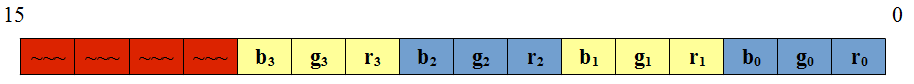
\includegraphics[scale=0.66]{imagenes/popart1.png}
  \caption{Estado inicial de XMM0}
  \label{fig:popart1}
  \end{center}
\end{figure}

Luego se aplica la operación \texttt{PSHUFB} para cada registro, con las
máscaras \textbf{<<MÁSCARA R>>}, \textbf{<<MÁSCARA G>>} y \textbf{<<MÁSCARA
B>>}, tal y como se puede apreciar en \fig{popart_mask_r} para rojo,
\fig{popart_mask_g} para verde y \fig{popart_mask_b} para azul respectivamente.
Luego de aplicar estas máscaras, como los valores fuente eran bytes sin signo,
se puede extenderlos simplemente agregando ceros adelante. Por la forma en que
están dispuestos los valores, esta extensión del tamaño del dato es trivial, tal
y como se ejemplifica en \fig{popart_extiende_r} para el color rojo. La misma
``operación'' (trivial, virtual) se realiza para el resto de los registros.

\begin{figure}[h]
  \begin{center}
  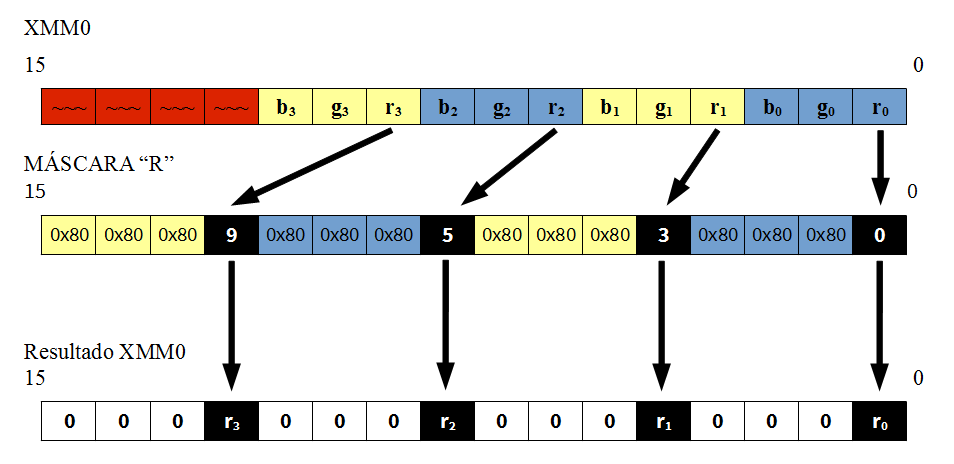
\includegraphics[scale=0.55]{imagenes/popart-mask-r.png}
  \caption{\textbf{<<MÁSCARA R>>}}
  \label{fig:popart_mask_r}
  \end{center}
\end{figure}

\begin{figure}[h]
  \begin{center}
  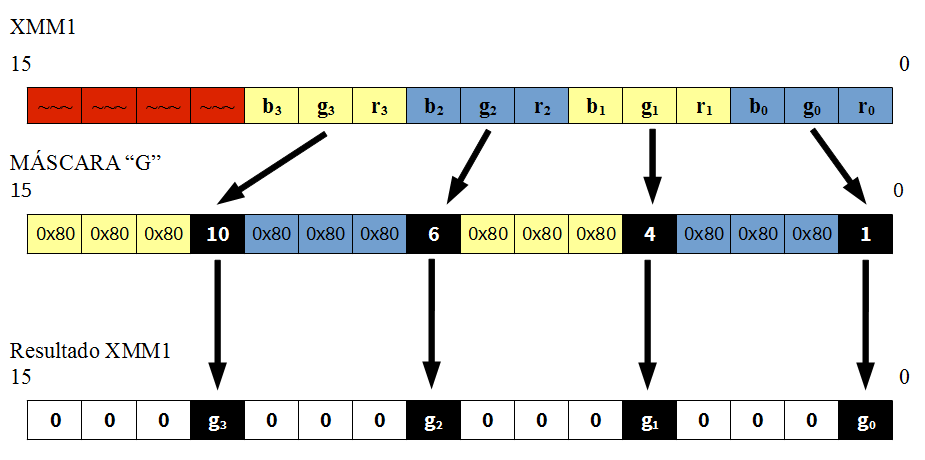
\includegraphics[scale=0.55]{imagenes/popart-mask-g.png}
  \caption{\textbf{<<MÁSCARA G>>}}
  \label{fig:popart_mask_g}
  \end{center}
\end{figure}

\begin{figure}[h]
  \begin{center}
  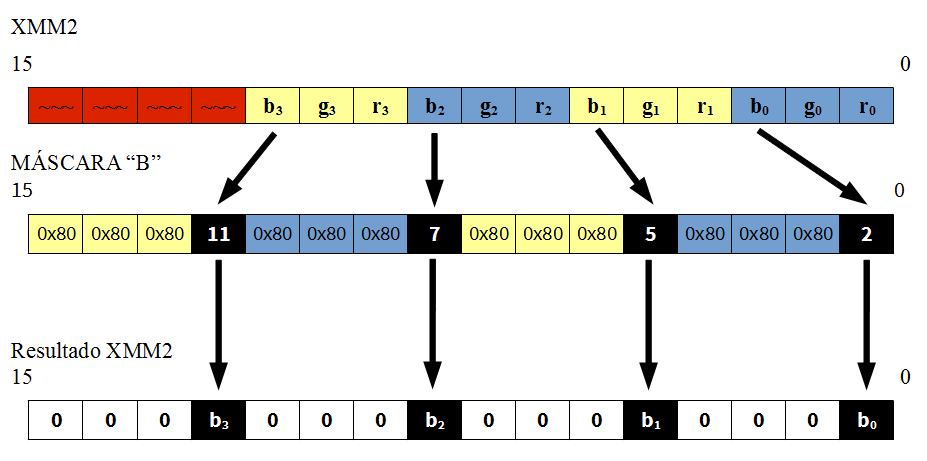
\includegraphics[scale=0.55]{imagenes/popart-mask-b.png}
  \caption{\textbf{<<MÁSCARA B>>}}
  \label{fig:popart_mask_b}
  \end{center}
\end{figure}

\begin{figure}[h]
  \begin{center}
  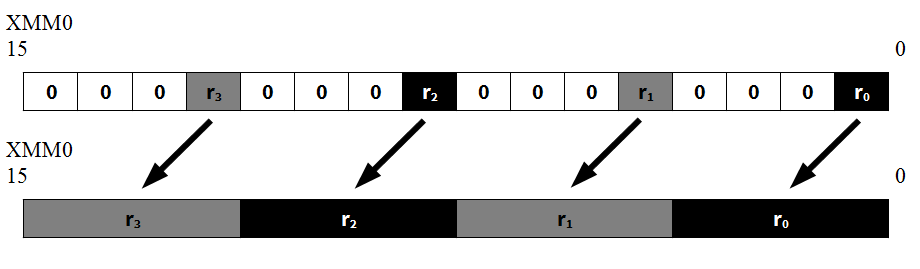
\includegraphics[scale=0.66]{imagenes/popart-extiende-r.png}
  \caption{Extiende el registro trivialmente}
  \label{fig:popart_extiende_r}
  \end{center}
\end{figure}



%\newpage
\clearpage

\vspace*{0.3cm} \noindent
\textbf{Experimento 2 - cpu vs. bus de memoria}

	¿Cuál es el factor que limita la performance en este caso? 
	
	Realizar un experimento, agregando múltiples instrucciones de un mismo tipo
	y realizar un análisis 	del resultado. Acompañar con un gráfico.


\vspace*{0.3cm} \noindent
\textbf{Experimento 3 - prefetch}

  La técnica de \textit{prefetch} es otra forma de optimización que puede
  realizarse. Su sustento teórico es el siguiente:
  
  Suponga un algoritmo que en cada iteración tarda n ciclos en obtener un dato y una cantidad
  similar en procesarlo. Si el algoritmo lee el dato $i$ y luego lo procesa,
  desperdiciará siempre n ciclos esperando entre que el dato llega y que se comienza
  a procesar efectivamente. Un algoritmo más inteligente podría pedir el 
  dato $i+1$ al comienzo del ciclo de proceso del dato $i$ (siempre suponiendo
  que el dato $i$ pidió en la iteración $i-1$. De esta manera, a la vez que el
  procesador computa todas las instrucciones de la iteración $i$, se estáran trayendo
  los datos de la siguiente iteración, y cuando esta última comience, los datos ya
  habrán llegado.

  \vspace*{0.2cm}
  Estudiar esta técnica y proponer una aplicación al código del filtro en la versión ASM.
  Programarla y analizar el resultado. ¿Vale la pena hacer prefetching?

\vspace*{0.3cm} \noindent
\textbf{Experimento 3 - secuencial vs. vectorial}

  Analizar cuales son las diferencias de performace entre las versiones de C y ASM. 
  Realizar gráficos que representen estas diferencias.


\subsection*{Filtro \textit{Temperature}}

  Programar el filtro \textit{Temperature} en lenguaje C y en en ASM haciendo uso de 
  las instrucciones vectoriales (\textbf{SSE}).


\vspace*{0.3cm} \noindent
\textbf{Experimento 1}

  Analizar cuales son las diferencias de performace entre las versiones de C y ASM. 
  Realizar gráficos que representen estas diferencias.



\subsection*{Filtro \textit{LDR}}
  Programar el filtro \textit{LDR} en lenguaje C y en
  ASM haciendo uso de las instrucciones \textbf{SSE}.

\vspace*{0.3cm} \noindent
\textbf{Descripción}

En este filtro se procesa de a un solo pixel en cada iteración del ciclo principal. Esto se debe a que para cada pixel no alcanza una lectura a
memoria; se deben leer los 24 pixeles a su alrededor, lo que insume 5 lecturas a memoria.
Primero se calcula la suma de las componentes r, g, y b de los pixeles circundantes. El valor máximo de esta suma es 5 * 5 * 255 * 3 = 19125 que 
ocupa 15 bits. Ésto nos obliga a extender cada componente r, g, b a word antes de sumar, para prevenir un overflow.

El valor máximo de una componente r, g, o b, es 255. El módulo de alfa tiene como valor máximo 255. Luego el dividendo tiene como valor máximo
absoluto 1243603125, que ocupa 31 bits. Como la mantisa de un float es de 24 bits, debemos guardarlo en un double, cuya mantisa es de 53 bits.
Debemos realizar tres divisiones, una para cada componente del pixel procesado. Como estamos trabajando con doubles, vamos a poder hacer dos
divisiones en una sola instrucción, y la tercera en otra instrucción. Para podr hacer las dos divisiones, vamos a replicar ciertos valores 
que nos interesan. 
En registros xmm, como double, vamos a tener:

$alfa | alfa$

$max | max$

$sumargb | sumargb$

$- | src_r$

$src_g | src_b$

Luego procedemos a hacer las respectivas multiplicaciones y divisiones. Ahora, para sumar $src_{(i,j)}$ y $var_{(i,j)}$, los voy a tener que
considerar como $signed$. Entonces, los voy a querer tener como signed word. $src_{(i,j)}$ lo voy a extender con ceros, y $var_{(i,j)}$, que era
de punto flotante, lo voy a truncar con signo. Se efectua una suma con signo, ahora podemos trabajar con r, g, y b al mismo tiempo. El resultado
se empaqueta de vuelta a byte, con saturación sin signo. Ahora se escribe el pixel procesado a memoria.

\vspace*{0.3cm} \noindent
\textbf{Experimento 1}

  Analizar cuales son las diferencias de performace entre las versiones de C y ASM. 
  Realizar gráficos que representen estas diferencias.



\section{Conclusiones y trabajo futuro}


\end{document}

